%
% Sección de modos de operación, capítulo de antecedentes.
% Proyecto Lovelace.
%

\subsection{Modos de operación}

Por sí solos, los cifrados por bloques solamente permiten el cifrado y
descifrado de bloques de información de tamaño fijo; donde, en la mayoría de
los casos, los bloques son de menos de 256 bits\cite{modos_de_operacion}, lo
cual es equivalente a alrededor de 8 caracteres. Es fácil darse cuenta de que
esta restricción no es ningún tema menor: en la gran mayoría de las
aplicaciones, la longitud de lo que se quiere ocultar es arbitraria.

Los \glspl{gl:modo_de_operacion} permiten extender la funcionalidad de los
cifrados por bloques para poder aplicarlos a información de tamaño irrestricto.
Se formaliza este concepto definiendo a un cifrado por bloques como una función
$ C $ (ecuación \ref{cifrado_por_bloques}) y a un \gls{gl:modo_de_operacion}
como una función $ M $ (ecuación \ref{modo_de_operacion}).

\begin{equation}
  \label{cifrado_por_bloques}
  C(L, B) \rightarrow Bc
\end{equation}

En donde $ L $ es la llave y $ B $ es el bloque a cifrar; ambos con un tamaño
definido: $ L \in \{0, 1\}^k $ ($ k $ es el tamaño de la llave) y
$ B \in \{0, 1\}^n $ ($ n $ es el tamaño de bloque). $ Bc $ representa al
bloque cifrado, el cuál también tiene longitud $ n $.

\begin{equation}
  \label{modo_de_operacion}
  M(L, T) \rightarrow Tc
\end{equation}

En este caso $ L $ es la misma que en \ref{cifrado_por_bloques}, $ T $ y
$ Tc $ son el texto original y el texto cifrado, respectivamente, y ambos
son de longitud arbitraria: $ T, Tc \in \{0, 1\}^* $.

Un primer enfoque (y quizás el más intuitivo) es partir el mensaje original
en bloques del tamaño requerido y después aplicar el algoritmo a cada bloque
por separado; en caso de que la longitud del mensaje no sea múltiplo del
tamaño de bloque, se puede agregar información extra al último bloque para
completar el tamaño requerido. Este es, de hecho, el primero de los modos que
se presentan a continuación, el \acrfull{gl:ecb}; su uso no es
recomendado, pues es muy inseguro cuando el mensaje original es simétrico a
nivel de bloque \cite{modos_de_operacion}. También se enlistan otros tres
modos, los cuales junto con \acrshort{gl:ecb}, son los más comunes.

% TODO: indagar un poco más en la inseguridad de ECB (dentro de su propia
% scción).

%
% Modo de operación ECB, capítulo de antecedentes.
% Proyecto Lovelace.
%

\subsubsection{\textit{Electronic Codebook} (ECB)}

La figura \ref{figura:ecb} muestra un diagrama esquemático de este
\gls{gl:modo_de_operacion}. El algoritmo recibe a la entrada una llave y un
mensaje de longitud arbitraria: la llave se pasa sin ninguna modificación a
cada función del cifrado por bloques; el mensaje se debe de partir en bloques
($ M = Bm_1 || Bm_2 || \dots || Bm_n $).

\begin{figure}
  \centering
  \begin{subfigure}{0.45\textwidth}
    \begin{center}
      \subimport{diagramas/}{modo_ecb.tikz.tex}
      \caption{Cifrado.}
    \end{center}
  \end{subfigure}
  \begin{subfigure}{0.45\textwidth}
    \begin{center}
      \subimport{diagramas/}{modo_ecb_inverso.tikz.tex}
      \caption{Descifrado.}
    \end{center}
  \end{subfigure}
  \caption{\Gls{gl:modo_de_operacion} \gls{gl:ecb}.}
  \label{figura:ecb}
\end{figure}

\begin{pseudocodigo}[%
    caption={\Gls{gl:modo_de_operacion} \gls{gl:ecb}, cifrado.}%
  ]
    entrada: llave $ k $; bloques de mensaje $ Bm_1, Bm_2 \dots Bm_n $.
    salida:  bloques de mensaje cifrado $ Bc_1, Bc_2 \dots Bc_n $.
    inicio
      para_todo $Bm$
        $Bc_i$ $\gets$ E_k($Bm_i$)
      fin
      regresar $Bc$
    fin
\end{pseudocodigo}

\begin{pseudocodigo}[%
    caption={\Gls{gl:modo_de_operacion} \gls{gl:ecb}, descifrado.}%
  ]
    entrada: llave $ k $; bloques de mensaje cifrado $ Bc_1, Bc_2 \dots Bc_n $.
    salida:  bloques de mensaje original $ B_1, B_2 \dots B_n $.
    inicio
      para_todo $Bc$
        $Bm_i$ $\gets$ $D_k$($Bc_i$)
      fin
      regresar $Bm$
    fin
\end{pseudocodigo}

%
% Modo de operación CBC, capítulo de antecedentes.
% Proyecto Lovelace.
%

\subsection{\textit{Cipher-block Chaining} (CBC)}

En CBC la salida del bloque cifrador uno se introduce (junto con el siguiente
bloque del mensaje) en el bloque cifrador dos, y así en sucesivo. Para poder
replicar este comportamiento en todos los bloque cifradores, este modo de
operación necesita un argumento extra a la entrada: un vector de
inicialización. De esta manera la salida del bloque $ i $ depende de todos
los bloques anteriores; esto incrementa la seguridad con respecto a ECB.

\vspace{0.5cm}

\begin{figure}[H]
  \centering
  \begin{subfigure}{0.45\textwidth}
      \begin{center}
          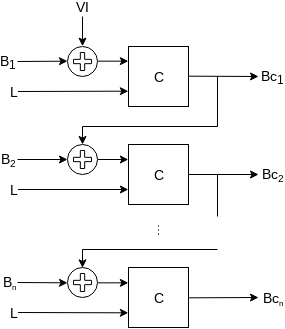
\includegraphics[width=0.7\linewidth]
            {contenidos/antecedentes/modos/diagramas/modo_cbc.png}
          \caption{Cifrado.}
      \end{center}
  \end{subfigure}
  \begin{subfigure}{0.45\textwidth}
      \begin{center}
          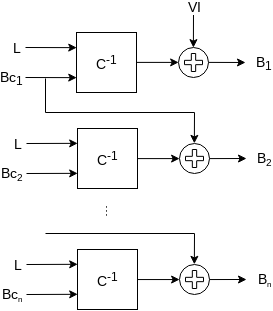
\includegraphics[width=0.7\linewidth]
            {contenidos/antecedentes/modos/diagramas/modo_cbc_inverso.png}
          \caption{Descifrado.}
      \end{center}
  \end{subfigure}
  \caption{Modo de operación CBC.}
  \label{figura:cbc}
\end{figure}

En la figura \ref{figura:cbc} se muestran los diagramas esquemáticos para
cifrar y descifrar; en los pseudocódigos \ref{cbc:1} y \ref{cbc:2} se muestran
unos de los posibles algoritmos a seguir. Es importante notar que mientras que
el proceso de cifrado debe ser forzosamente secuencial (por la dependencias
entre salidas), el proceso de descifrado puede ser ejecutado en paralelo.

\vspace{0.5cm}

% Látima que con los escapes en modo matemático dentro de los pseudocódigos
% se pierda totalmente la ventaja de trabajar con fuentes mono: por eso
% la alineación tan rara de los comentarios del próximo pseudocódigo.

\begin{pseudocodigo}[caption={Modo de operación CBC, cifrado.}, label={cbc:1}]
  entrada: llave $ L $; vector de inicialización $ VI $;
           bloques de mensaje $ B_1, B_2 \dots B_n $.
   salida: bloques de mensaje cifrado $ Bc_1, Bc_2 \dots Bc_n $.
  inicio
    $Bc_0$ $\gets$ $ VI $                         // El vector de incialización
    para_todo $B$                 // entra al primer bloque.
      $Bc_i$ $\gets$ C($L$, $B_i \oplus Bc_{i - 1}$)
    fin
    regresar $Bc$
  fin
\end{pseudocodigo}

\begin{pseudocodigo}[caption={Modo de operación CBC, descifrado.}, label={cbc:2}]
  entrada: llave $ L $; vector de inicialización $ VI $;
           bloques de mensaje cifrado $ Bc_1, Bc_2 \dots Bc_n $.
   salida: bloques de mensaje original $ B_1, B_2 \dots B_n $.
  inicio
    $Bc_0$ $\gets$ $ VI $
    para_todo $Bc$
      $B_i$ $\gets$ $C^{-1}$($L$, $Bc_i$) $\oplus$ $Bc_{i-1}$
    fin
    regresar $B$
  fin
\end{pseudocodigo}

%
% Modo de operación CFB, capítulo de antecedentes.
% Proyecto Lovelace.
%

\subsubsection{\textit{Cipher Feedback} (CFB)}

Al igual que la operación de cifrado de \gls{gl:cbc}, ambas operaciones
de \gls{gl:cfb} (cifrado y descifrado) están encadenadas bloque a bloque,
por lo que son de naturaleza secuencial. En este caso, lo que se cifra en el
primer paso es el \gls{gl:vector_de_inicializacion}; la salida de esto se opera
con un \verb|xor| sobre el primer bloque de texto en claro, para obtener el
primer bloque cifrado (figura \ref{fig:cfb}).

Esta distribución presenta varias ventajas con respecto a \gls{gl:cbc}:
las operaciones de cifrado y descifrado son sumamente similares, lo que permite
ser implementadas por un solo algoritmo (pseudocódigo \ref{cfb:1}); tanto para
cifrar como para descifrar solamente se ocupa la operación de cifrado del
algoritmo a bloques subyacente. Estas ventajas se deben principalmente a las
propiedades de la operación \verb|xor| (ecuación \ref{xor:inverso_igual}).

\begin{equation}
  \label{xor:inverso_igual}
  A \oplus B = C \quad \Rightarrow \quad A = B \oplus C
\end{equation}

\begin{figure}[H]
  \centering
  \begin{subfigure}{0.45\textwidth}
    \begin{center}
      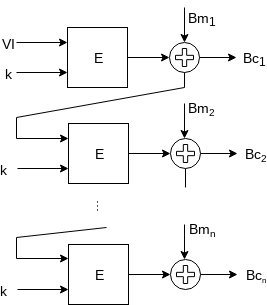
\includegraphics[width=0.6\linewidth]
        {contenidos/antecedentes/bloques/modos/diagramas/modo_cfb.png}
      \caption{Cifrado.}
    \end{center}
  \end{subfigure}
  \begin{subfigure}{0.45\textwidth}
    \begin{center}
      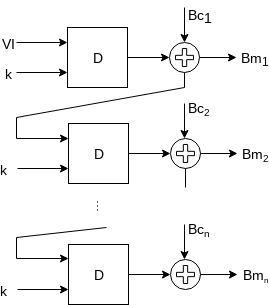
\includegraphics[width=0.6\linewidth]
        {contenidos/antecedentes/bloques/modos/diagramas/modo_cfb_inverso.png}
      \caption{Descifrado.}
    \end{center}
  \end{subfigure}
  \caption{\Gls{gl:modo_de_operacion} \gls{gl:cfb}.}
  \label{fig:cfb}
\end{figure}

\begin{pseudocodigo}[%
    caption={\Gls{gl:modo_de_operacion} \gls{gl:cfb}%
      (cifrado y descifrado).},
    label={cfb:1}%
  ]
  entrada: llave $ k $; vector de inicialización $ VI $;
           bloques de mensaje (cifrado o descifrado) $ Bm_1, Bm_2 \dots Bm_n $.
  salida:  bloques de mensaje (cifrado o descifrado) $ Bc_1, Bc_2 \dots Bc_n $.
  inicio
    $Bc_0$ $\gets$ $ VI $
    para_todo $Bm$
      $Bc_i$ $\gets$ $C_k$($Bc_{i - 1}$) $\oplus$ $Bm_i$
    fin
    regresar $Bc$
  fin
\end{pseudocodigo}

%
% Modo de operación OFB, capítulo de antecedentes.
% Proyecto Lovelace.
%

\newpage
\subsection{\textit{Output Feedback} (OFB)}

Este es muy similar al anterior (CFB), salvo porque la retroalimentación va
directamente de la salida del cifrador a bloques. De esta forma, nada que
tenga que ver con el texto en claro, llega al cifrado a bloques; este
solamente se la pasa cifrando una y otra vez el vector de inicialización.

\vspace{0.5cm}

\begin{figure}[H]
  \centering
  \begin{subfigure}{0.45\textwidth}
      \begin{center}
          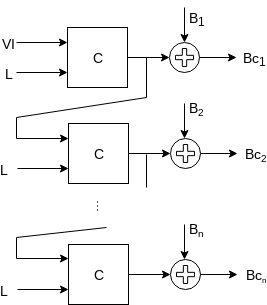
\includegraphics[width=0.7\linewidth]
            {contenidos/antecedentes/modos/diagramas/modo_ofb.png}
          \caption{Cifrado.}
      \end{center}
  \end{subfigure}
  \begin{subfigure}{0.45\textwidth}
      \begin{center}
          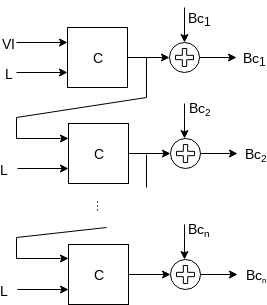
\includegraphics[width=0.7\linewidth]
            {contenidos/antecedentes/modos/diagramas/modo_ofb_inverso.png}
          \caption{Descifrado.}
      \end{center}
  \end{subfigure}
  \caption{Modo de operación OFB.}
\end{figure}

\begin{pseudocodigo}[caption={Modo de operación OFB (cifrado y descifrado).}]
  entrada: llave $ L $; vector de inicialización $ VI $;
           bloques de mensaje (cifrado o descifrado) $ B_1, B_2 \dots B_n $.
   salida: bloques de mensaje (cifrado o descifrado) $ Bc_1, Bc_2 \dots Bc_n $.
  inicio
    aux $\gets$ $ VI $
    para_todo $B$
      aux $\gets$ C($L$, aux)
      $Bc_i$ $\gets$  aux $\oplus$ $B_i$
    fin
    regresar $Bc$
  fin
\end{pseudocodigo}

